%%%%%%%%%%%%%%%%%%%%%%%%%%%%%%%%%%%%%%%%%%%%%%%%%%%%%%%%%%%%%%%%%%
%%%%%%%%%%%%%%%%%%%%%%%%%%%%%%%%%%%%%%%%%%%%%%%%%%%%%%%%%%%%%%%%%%
%Packages
\documentclass[10pt, a4paper]{article}
\usepackage{naturetex}
\usepackage[normalem]{ulem}
\usepackage[top=3cm, bottom=4cm, left=3.5cm, right=3.5cm]{geometry}
\usepackage{amsmath,amsthm,amsfonts,amssymb,amscd, fancyhdr, color, comment, graphicx, environ}
\usepackage{float}
\usepackage{graphicx}
%\usepackage[table,xcdraw]{xcolor}
\usepackage{mathrsfs}
\usepackage[math-style=ISO]{unicode-math}
\setmathfont{TeX Gyre Termes Math}
\usepackage{lastpage}
\usepackage[dvipsnames]{xcolor}
\usepackage[framemethod=TikZ]{mdframed}
\usepackage{multirow}
\usepackage{enumerate}
\usepackage[shortlabels]{enumitem}
\usepackage{ctex}
\usepackage{fancyhdr}
\usepackage{indentfirst}
\usepackage{listings}
\usepackage{sectsty}
\usepackage{thmtools}
\usepackage{shadethm}
\usepackage{hyperref}
\usepackage{setspace}
\hypersetup{
	colorlinks=true,
	linkcolor=blue,
	filecolor=magenta,      
	urlcolor=blue,
}
%%%%%%%%%%%%%%%%%%%%%%%%%%%%%%%%%%%%%%%%%%%%%%%%%%%%%%%%%%%%%%%%%%
%%%%%%%%%%%%%%%%%%%%%%%%%%%%%%%%%%%%%%%%%%%%%%%%%%%%%%%%%%%%%%%%%%
%Environment setup
\mdfsetup{skipabove=\topskip,skipbelow=\topskip}
\newrobustcmd\ExampleText{%
	An \textit{inhomogeneous linear} differential equation has the form
	\begin{align}
		L[v ] = f,
	\end{align}
	where $L$ is a linear differential operator, $v$ is the dependent
	variable, and $f$ is a given non−zero function of the independent
	variables alone.
}

\mdtheorem[style=theoremstyle]{Problem}{Problem}
\newenvironment{Solution}{\textbf{Solution.}}

%%%%%%%%%%%%%%%%%%%%%%%%%%%%%%%%%%%%%%%%%%%%%%%%%%%%%%%%%%%%%%%%%%
%%%%%%%%%%%%%%%%%%%%%%%%%%%%%%%%%%%%%%%%%%%%%%%%%%%%%%%%%%%%%%%%%%
%Fill in the appropriate information below
\newcommand{\norm}[1]{\left\lVert#1\right\rVert}     
\newcommand\course{Course}                      % <-- course name   
\newcommand\hwnumber{1}                         % <-- homework number
\newcommand\Information{XXX/xxxxxxxx}           % <-- personal information
%%%%%%%%%%%%%%%%%%%%%%%%%%%%%%%%%%%%%%%%%%%%%%%%%%%%%%%%%%%%%%%%%%
%%%%%%%%%%%%%%%%%%%%%%%%%%%%%%%%%%%%%%%%%%%%%%%%%%%%%%%%%%%%%%%%%%
%Page setup
\pagestyle{fancy}
\headheight 40pt
\lhead{\today}
\rhead{
\includegraphics[width=2.5cm]{西安交通大学logo2}} % <-- school logo(please upload the file first, then change the name here)
\lfoot{}
\pagenumbering{arabic}
\cfoot{\small\thepage}
\rfoot{}
\headsep 1.25em
\renewcommand{\baselinestretch}{1.25}       
\mdfdefinestyle{theoremstyle}{%
	linecolor=black,linewidth=1pt,%
	frametitlerule=true,%
	frametitlebackgroundcolor=gray!20,
	innertopmargin=\topskip,
}
%%%%%%%%%%%%%%%%%%%%%%%%%%%%%%%%%%%%%%%%%%%%%%%%%%%%%%%%%%%%%%%%%%
%%%%%%%%%%%%%%%%%%%%%%%%%%%%%%%%%%%%%%%%%%%%%%%%%%%%%%%%%%%%%%%%%%
%Add new commands here
\renewcommand{\labelenumi}{\alph{enumi})}
\newcommand{\Z}{\mathbb Z}
\newcommand{\R}{\mathbb R}
\newcommand{\Q}{\mathbb Q}
\newcommand{\NN}{\mathbb N}
\DeclareMathOperator{\Mod}{Mod} 
\renewcommand\lstlistingname{Algorithm}
\renewcommand\lstlistlistingname{Algorithms}
\def\lstlistingautorefname{Alg.}
%%%%%%%%%%%%%%%%%%%%%%%%%%%%%%%%%%%%%%%%%%%%%%%%%%%%%%%%%%%%%%%%%%
%%%%%%%%%%%%%%%%%%%%%%%%%%%%%%%%%%%%%%%%%%%%%%%%%%%%%%%%%%%%%%%%%%
%Begin now!



\begin{document}
	
	\begin{titlepage}
		\begin{center}
			\vspace*{3cm}
			
			\Huge
			\textbf{《社交网络和文本分析》大作业}
			
			\vspace{1cm}
	
			\vspace{3.5cm}
					
\includegraphics[width=0.7\textwidth]{西安交通大学logo2}
			
			\vfill
			
			
			\Large
			\begin{center}
				\begin{tabular}{rl}
					% after \\: \hline or \cline{col1-col2} \cline{col3-col4} ...
					\textbf{学号:}& 2193712622\\
					\textbf{姓名:}& 赵敬业\\
					\textbf{班级:}& 大数据01\\

				\end{tabular}
			\end{center}




			
			\Large
			
			\today
			
		\end{center}
	\end{titlepage}
	
	%%%%%%%%%%%%%%%%%%%%%%%%%%%%%%%%%%%%%%%%%%%%%%%%%%%%%%%%%%%%%%%%%%
	%%%%%%%%%%%%%%%%%%%%%%%%%%%%%%%%%%%%%%%%%%%%%%%%%%%%%%%%%%%%%%%%%%
	%Start the assignment now
	
	%%%%%%%%%%%%%%%%%%%%%%%%%%%%%%%%%%%%%%%%%%%%%%%%%%%%%%%%%%%%%%%%%%
	%New problem
% 目录
\newpage
\tableofcontents
\newpage

\section{社交网络——LastFM亚洲用户分析}

Last.fm (如图\ref{fig:lastfm})是一个于 2002 年在英国成立的音乐网站。\cite{ContributorstoWikimediaprojects2022Jun}使用名为“Audioscrobbler”的音乐推荐系统,Last.fm 通过记录用户收听的曲目的详细信息来构建每个用户音乐品味的详细档案,无论是从互联网广播电台,或用户的计算机或许多便携式音乐设备。 此信息通过音乐播放器(其中包括Spotify、Deezer、Tidal、MusicBee、SoundCloud 和 Anghami)或通过安装在用户音乐播放器中的插件传输(“scrobbled”)到 Last.fm 的数据库。然后将数据显示在用户的个人资料页面上,并进行编译以创建个人艺术家的参考页面。

\begin{figure}[tbph!]
	\centering
	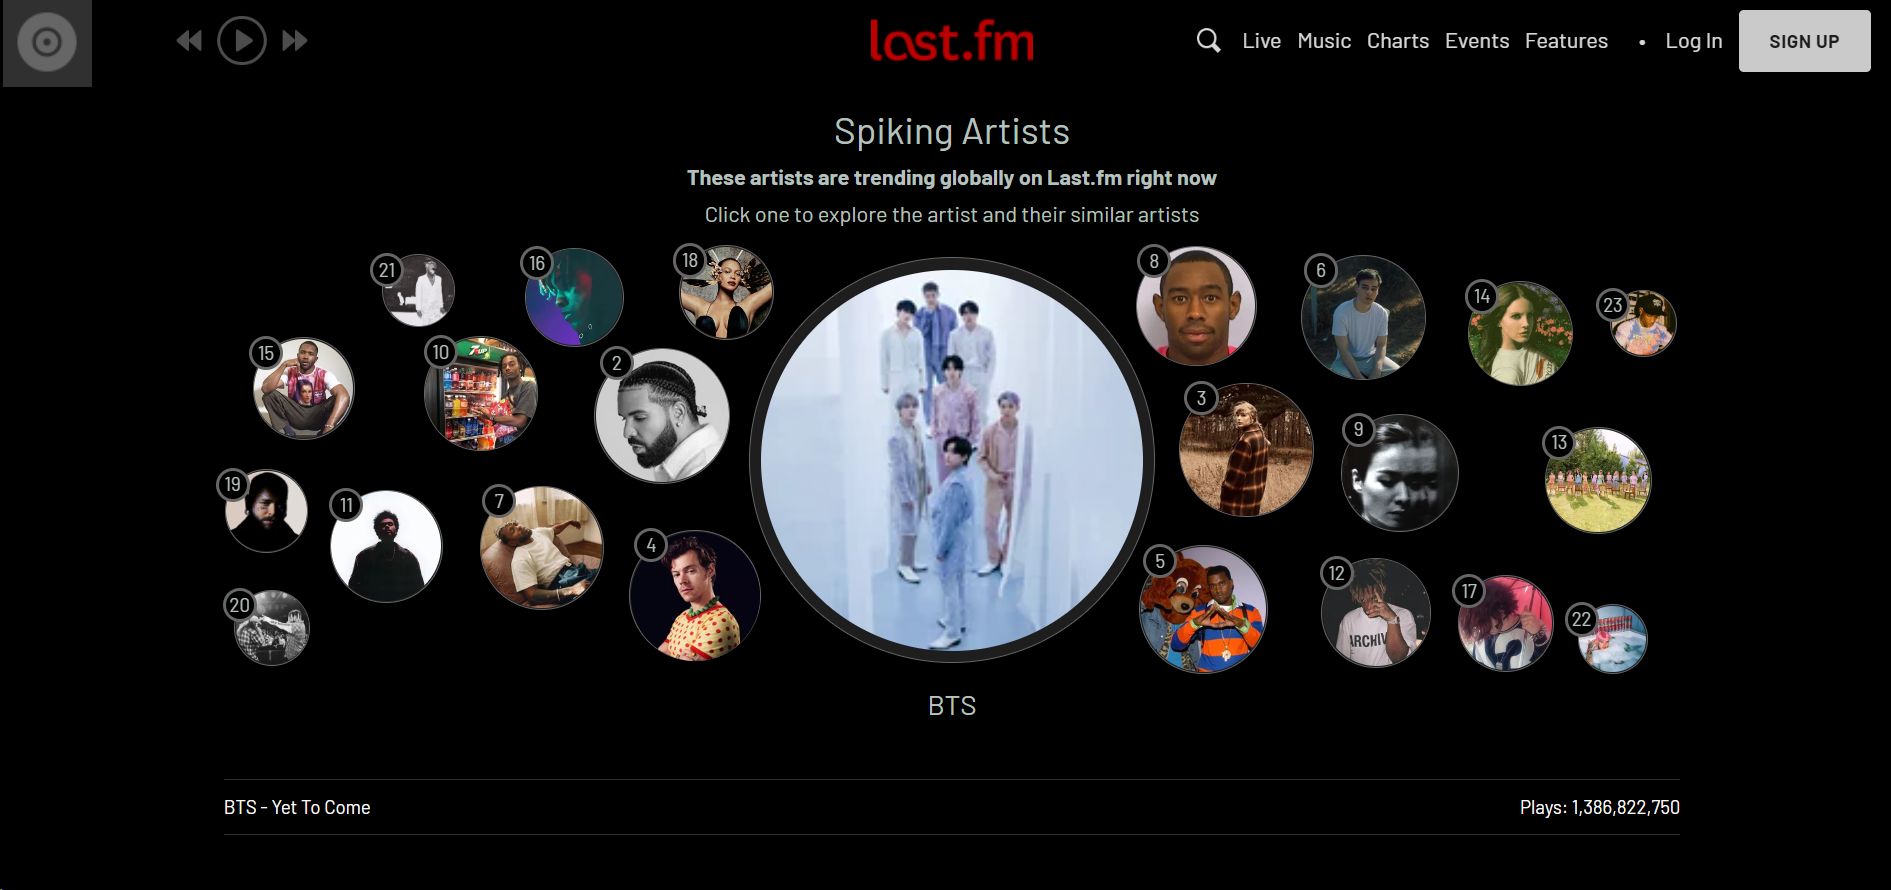
\includegraphics[width=0.7\linewidth]{figures/LastFM主页}
	\caption{LastFM主页}
	\label{fig:lastfm}
\end{figure}

本数据集\cite{rozemberczki2020characteristic}是2020 年 3 月从公共 API 收集的 LastFM 用户社交网络。节点是来自亚洲国家的 LastFM 用户,边是它们之间的相互追随者关系。统计信息如表格\ref{tab:st-of-social}

% Please add the following required packages to your document preamble:
% \usepackage{graphicx}
% \usepackage[table,xcdraw]{xcolor}
% If you use beamer only pass "xcolor=table" option, i.e. \documentclass[xcolor=table]{beamer}
\begin{table}[!htbp]
	\centering
		\begin{tabular}{ll}
			\hline
			节点  & 7,624                          \\
			边   & 27,806 \\
			密度  & 0.0009 \\
			传递性 & 0.1787\\
			\hline
		\end{tabular}%
	\caption{社交网络统计信息}
	\label{tab:st-of-social}
\end{table}

网络图可视化如图\ref{fig:raw-graph}。

\begin{figure}[tbph!]
	\centering
	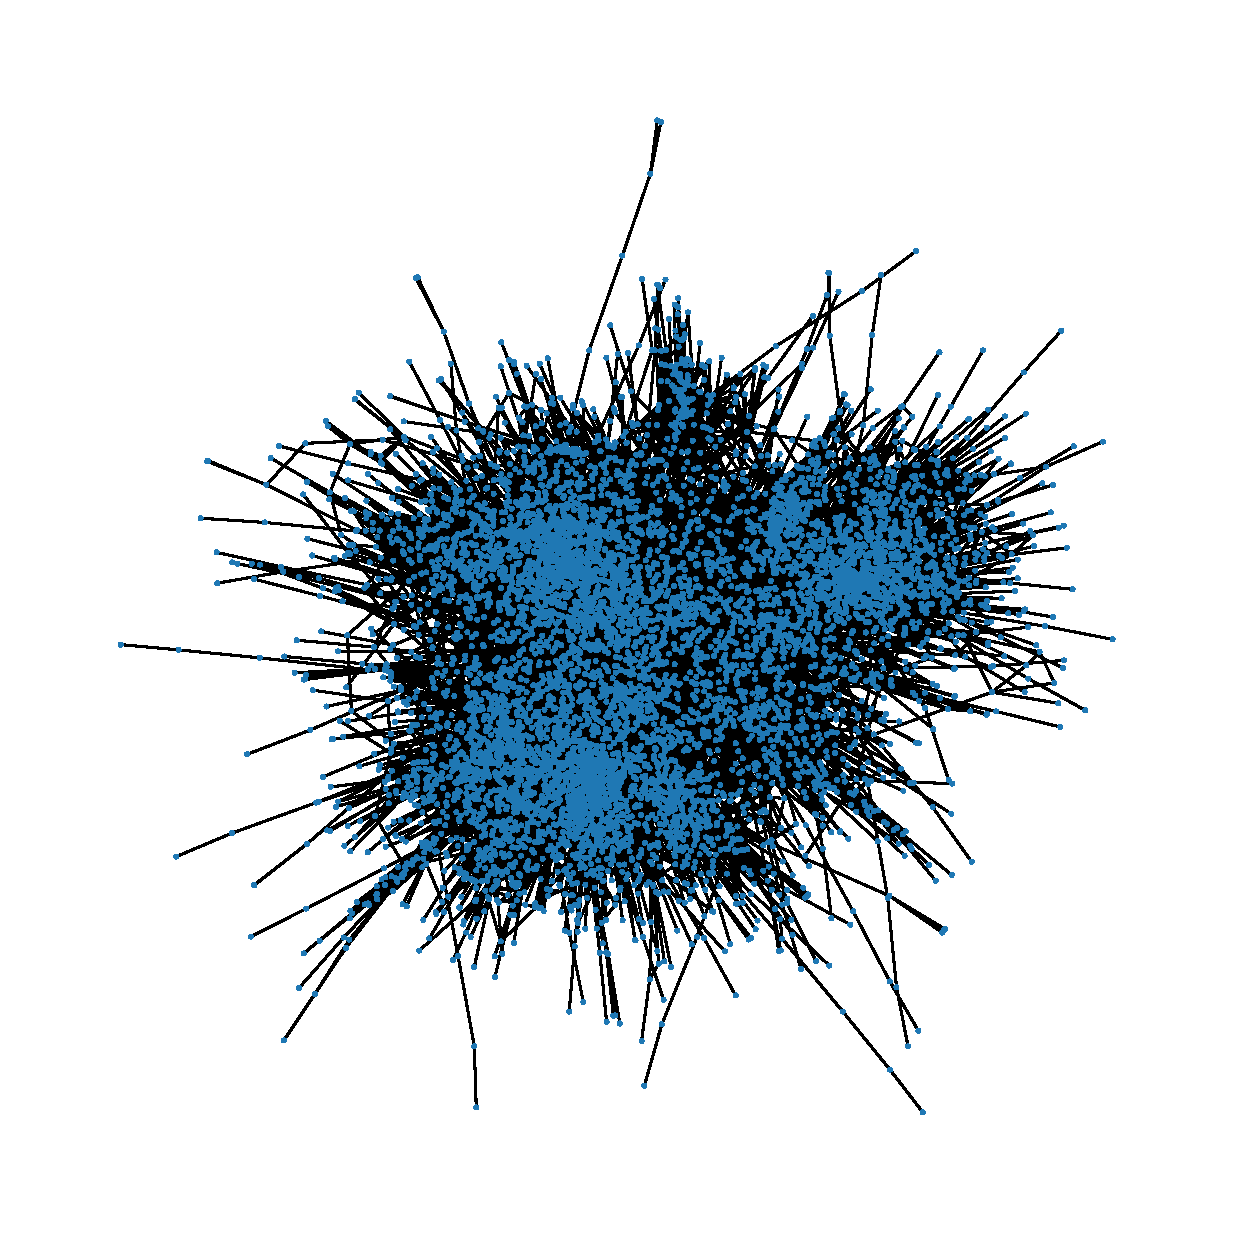
\includegraphics[width=0.7\linewidth]{figures/网络图}
	\caption{网络图}
	\label{fig:raw-graph}
\end{figure}

\subsection{节点重要性}

为了探索哪个节点更为重要,在本节使用度中心性、介数中心性、接近中心性、K核层数、特征向量大小以及PageRank指标进行探索。

度中心性通过一个节点连边的多少来进行衡量,一个节点连边越多,则度中心性越大。如图\ref{fig:度中心性}反映了网络中节点度中心性的分布规律,这是明显的幂律分布。

\begin{figure}[tbph!]
	\centering
	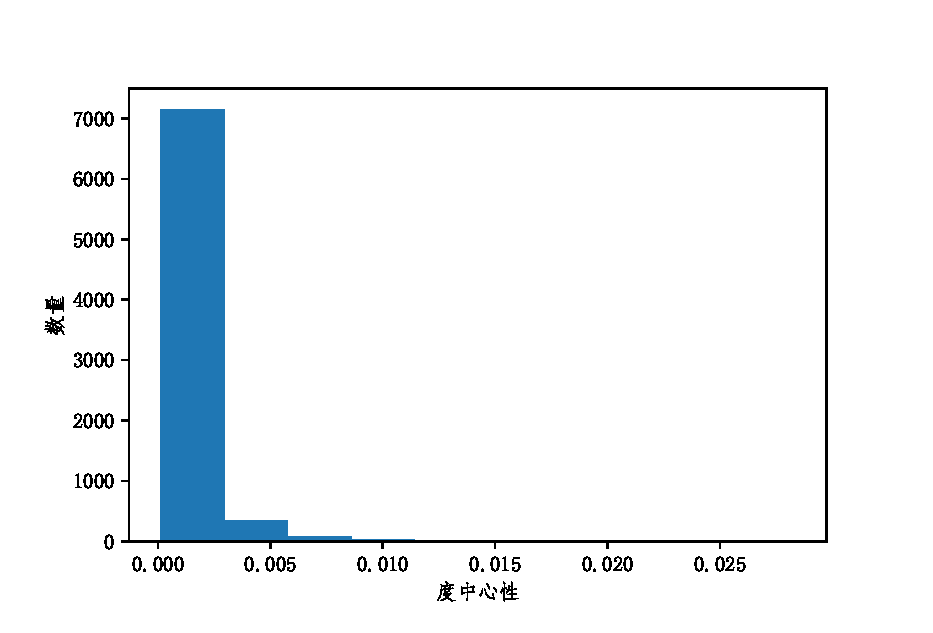
\includegraphics[width=0.5\linewidth]{figures/度中心性}
	\caption{度中心性统计结果}
	\label{fig:度中心性}
\end{figure}

介数中心性从最短路径的角度来判断节点的重要性,介数中心性大的节点在使图联系的更加紧密的作用越大,是一种判断节点重要性的理想指标。

\begin{figure}[tbph!]
	\centering
	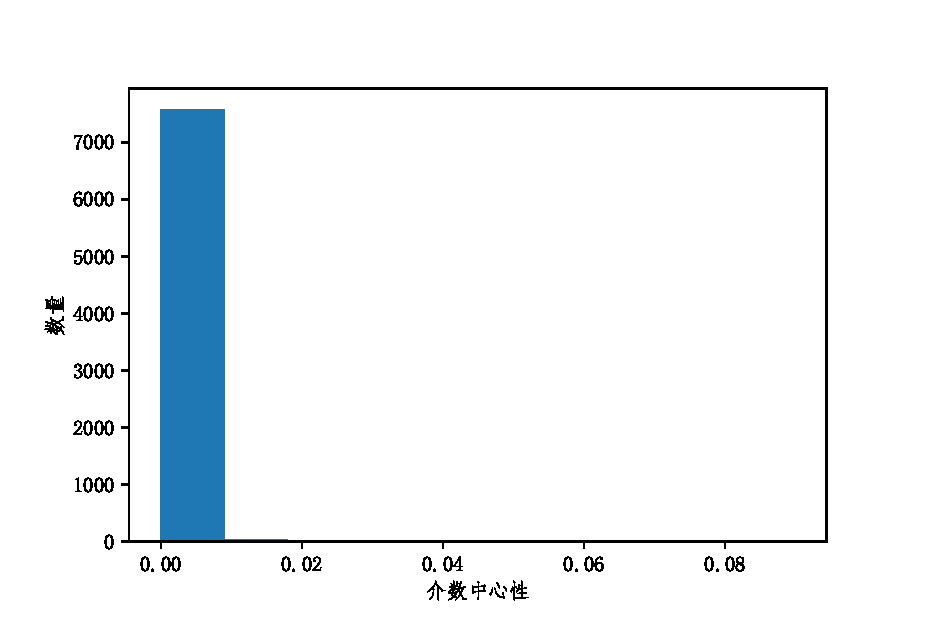
\includegraphics[width=0.5\linewidth]{figures/介数中心性}
	\caption{介数中心性统计结果}
	\label{fig:介数中心性}
\end{figure}
\begin{figure}[tbph!]
	\centering
	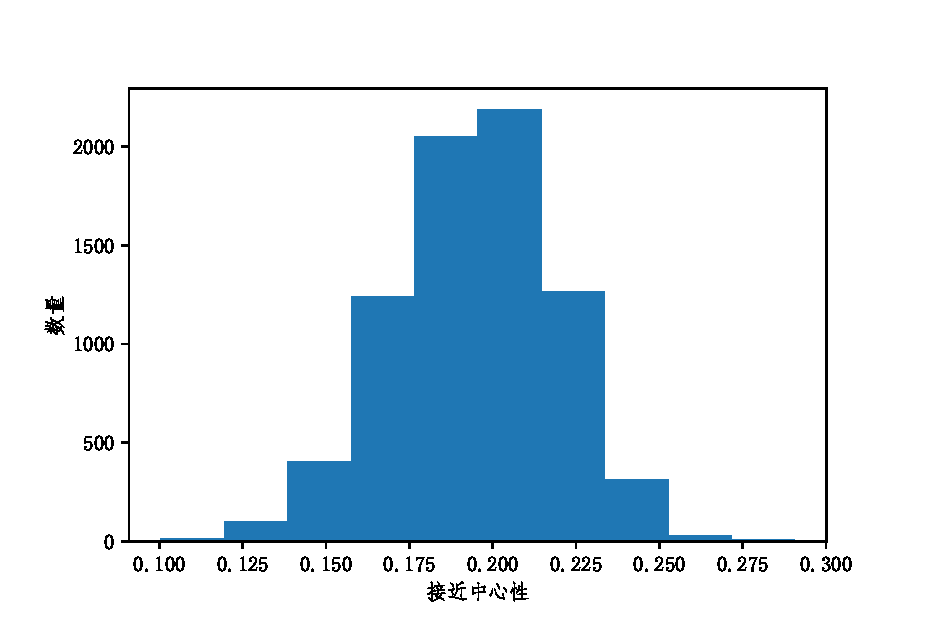
\includegraphics[width=0.5\linewidth]{figures/接近中心性}
	\caption{接近中心性统计结果}
	\label{fig:接近中心性}
\end{figure}
接近中心性是节点i与其它所有节点的平均距离。一个点的接近中心度较高,说明该点到网络中其他各点的距离总体来说较近,反之则较远。假如一个物流仓库网络需要选某个仓库作为核心中转站,需要它到其他仓库的距离总体来说最近,那么一种方法就是找到接近中心度最高的那个仓库。

K-核可以用来识别一个网络图中的核心成员。如图\ref{fig:K-core中心性}

\begin{figure}[tbph!]
	\centering
	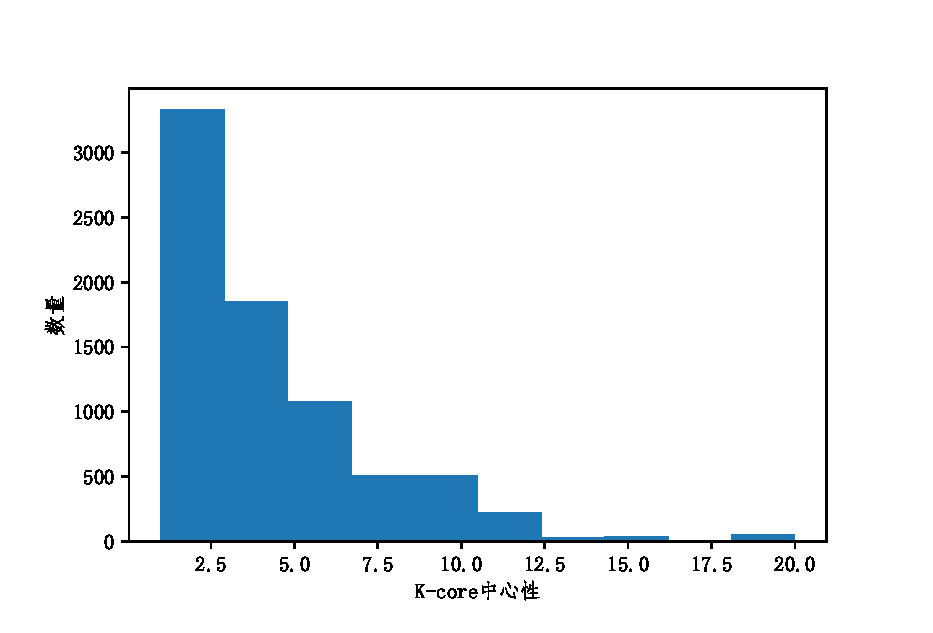
\includegraphics[width=0.5\linewidth]{figures/K-core中心性}
	\caption{K-core中心性统计结果}
	\label{fig:K-core中心性}
\end{figure}

特征向量中心性综合了本节点的重要性,也考虑了所有邻居节点的重要性,最终可以用特征向量的形式来解释该节点。如图\ref{label}

Page-Rank通过模拟一个漫游者,度量指向该节点的连接数,计算其中心性。
\begin{figure}[tbph!]
	\centering
	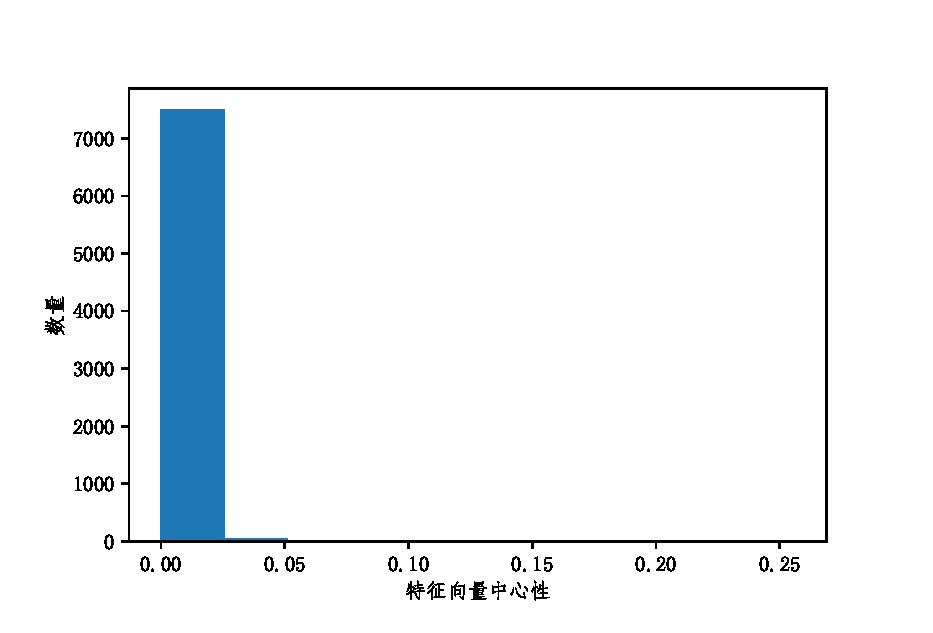
\includegraphics[width=0.5\linewidth]{figures/特征向量中心性}
	\caption{特征向量中心性统计结果}
	\label{fig:特征向量中心性}
\end{figure}
\begin{figure}[tbph!]
\centering
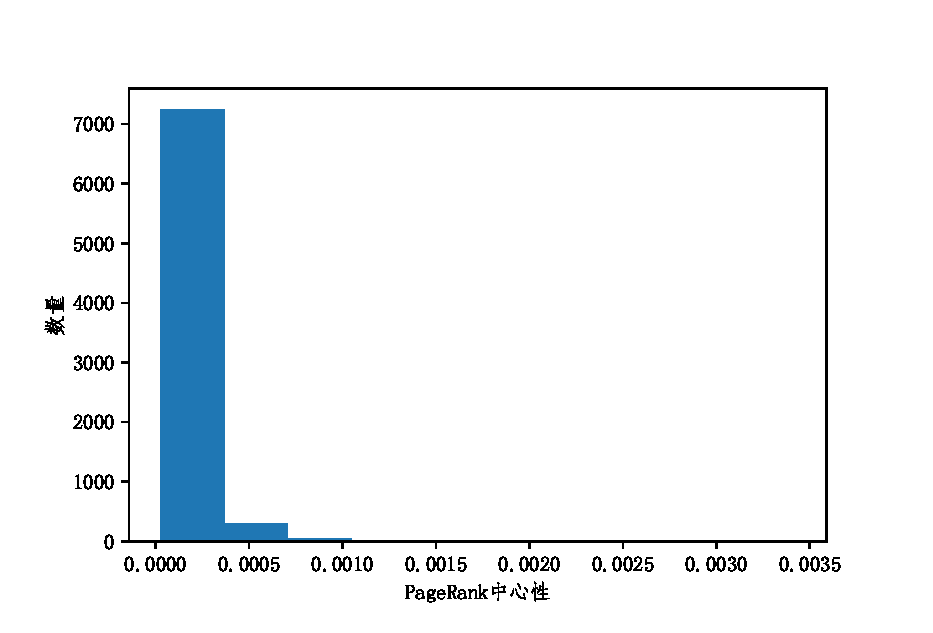
\includegraphics[width=0.5\linewidth]{figures/PageRank中心性}
\caption{PageRank中心性统计结果}
\label{fig:PageRank中心性}
\end{figure}

最终各种指标寻找的最重要的3个节点如表格\ref{tab:res-center},不同的指标得到的结果有所不同。

% Please add the following required packages to your document preamble:
% \usepackage{multirow}
% \usepackage[table,xcdraw]{xcolor}
% If you use beamer only pass "xcolor=table" option, i.e. \documentclass[xcolor=table]{beamer}
\begin{table}[!htbp]
	\centering
	\begin{tabular}{lll}
		\hline 
		指标                                                                          & 最重要节点名称                      & 节点重要性    \\
		\hline 
		&7237 & 0.028335 \\
		& 3530 & 0.022957 \\
		\multirow{-3}{*}{\begin{tabular}[c]{@{}l@{}}度中\\ 心性\end{tabular}} & 
		4785 & 0.022826 \\
		\hline
		& 7199                         & 0.089931 \\
		& 7237                         & 0.085589 \\
		\multirow{-3}{*}{\begin{tabular}[c]{@{}l@{}}介数\\ 中心性\end{tabular}} & 2854                         & 0.077563 \\
		\hline 
		& 7199                         & 0.290710 \\
		& 7237                         & 0.285677 \\
		\multirow{-3}{*}{\begin{tabular}[c]{@{}l@{}}接近\\ 中心性\end{tabular}} & 4356                         & 0.281603 \\
		\hline 
		& 427                          & 20       \\
		& 3240                         & 20       \\
		\multirow{-3}{*}{\begin{tabular}[c]{@{}l@{}}K核\\ 层 数\end{tabular}}     & 1348                         & 20       \\
		\hline 
		& 7237                         & 0.256134 \\
		& 3240                         & 0.196578 \\
		\multirow{-3}{*}{\begin{tabular}[c]{@{}l@{}}特征\\ 向 量\end{tabular}}     & 3597                         & 0.190829 \\
		\hline 
		& 4811                         & 0.003421 \\
		& 4785                         & 0.003261 \\
		\multirow{-3}{*}{PageRank}                                                  & 3530                         & 0.002719\\
	\end{tabular}
	\caption{不同重要性指标下最重要的三个节点}
	\label{tab:res-center}
\end{table}
\subsection{节点相似性指标}

本节通过节点相似度的计算尝试向ID为1的用户推荐好友。节点相似度是指计算节点相似性的方法。链路预测是节点相似度的一种应用。具体是将网络中的边分为两部分,一部分为训练集,一部分为测试集,构建预测模型,查看预测的准确性;好友推荐是节点相似度的另一种应用。具体是在Ego Network中,给Ego推荐潜在的好友。

节点相似度度量的原理是三元闭包原则。社会网络分析中三元闭包(Triadic closure)原则指出,如果两个人A和B拥有一个共同的朋友C,那么这两个人今后也很有可能成为朋友,从而使三个节点构成一个闭合的三角形ABC。对于一般的网络,这一原则推广如下:如果两个节点的共同邻居的数量越多,这两个节点就越相似,从而更倾向于互相连接。

AA指标\ref{eq:AA}在三元闭包原则的基础上提出,同时考虑了对共同好友进行加权的原则,在社交网络的好友推荐中有着广泛的应用。
\begin{align}\label{eq:AA}
	s_{xy}^{AA}=\sum_{z\in \Gamma(x)\bigcap\Gamma(y)}\frac{1}{\log k(z)}
\end{align}

除此之外,还尝试在AA指标的基础上进行改进,获得新的推荐好友的指标。考虑到AA指标充分利用了共同好友数的信息,但没有利用网络的拓扑结构,故在这个基础上进行改进,前往提到K核可以挖掘网络中节点的重要性,又考虑到处于同一网络层级的人可能更加倾向于有共同特点,从而更倾向于添加好友,故在AA指标的基础上除以两个人处于核层数的插值,称为SMX指标,如公式\ref{eq:SMX},新的指标随着两者所处的核层级数差异变大变小,反映了网络的拓扑结构。
\begin{align}\label{eq:SMX}
	s_{xy}^{SMX}=\frac{s_{xy}^{AA}}{|x_{core}-y_{core}|+1}
\end{align}


\subsection{挖掘社团结构}

为了将社团合理分类,此处使用几种算法来挖掘社团结构。

首先是对原始网络进行KMeans聚类。结果如图\ref{fig:KMeans}。对原始图片节点分成了四个类别,在图中用不同颜色来标记这些节点,其中大部分为蓝色,并且其他颜色的节点在网络中十分分散,可见效果并不很好。

\begin{figure}[tbph!]
	\centering
	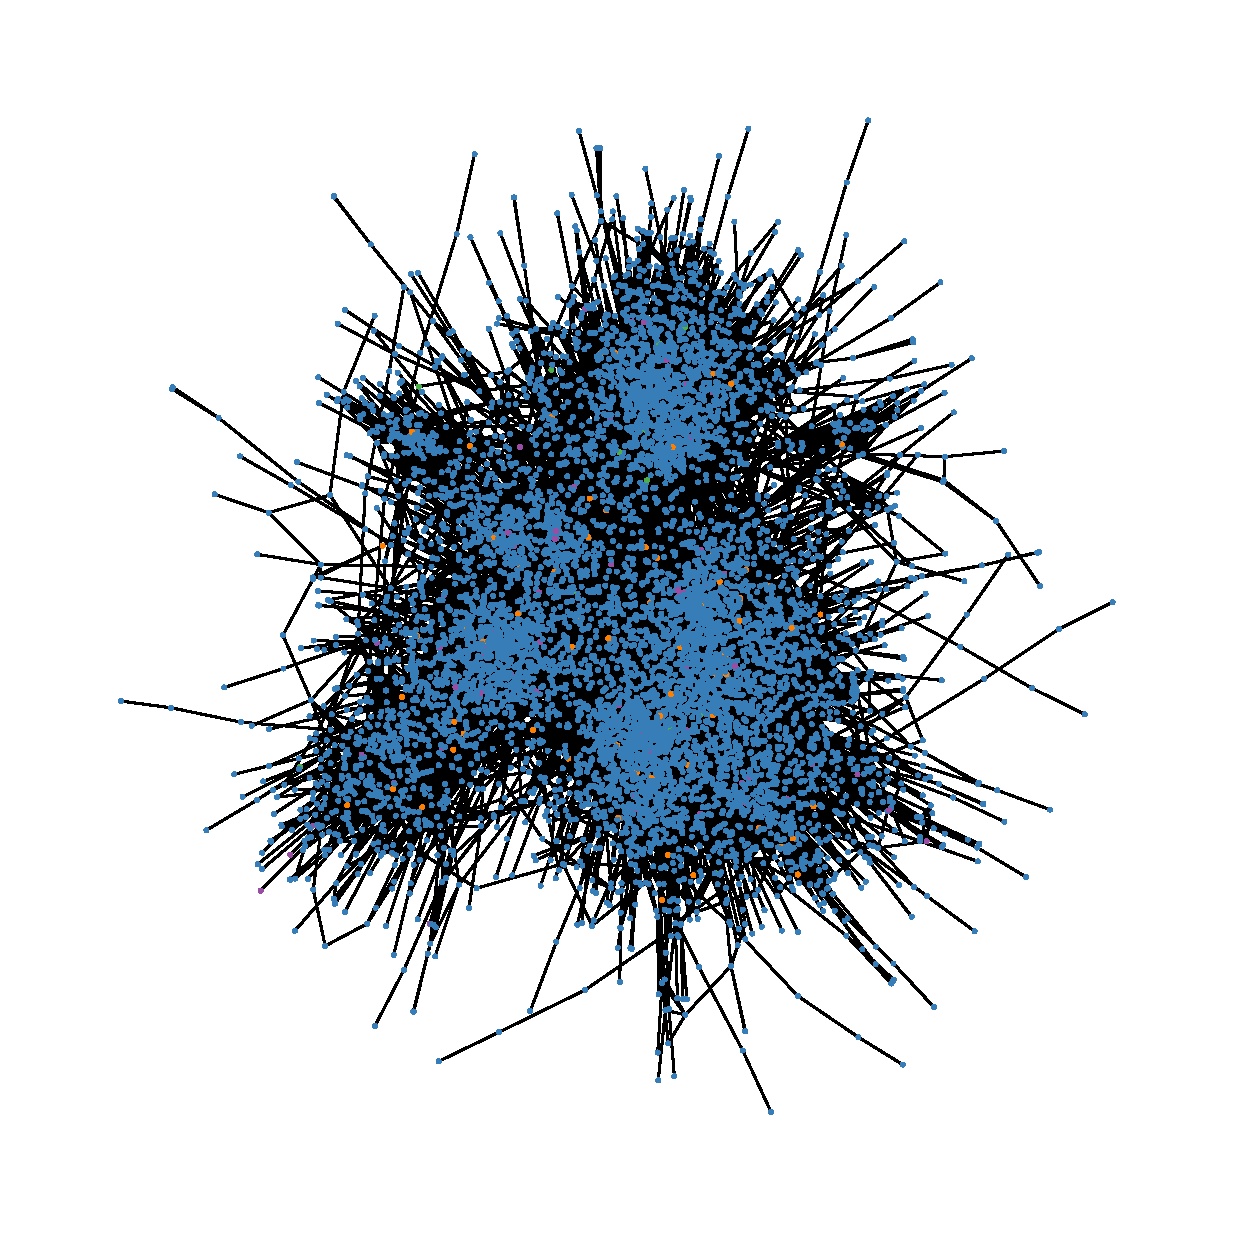
\includegraphics[width=0.5\linewidth]{figures/KMeans聚类结果}
	\caption{KMeans聚类结果}
	\label{fig:KMeans}
\end{figure}

之后尝试使用贪婪算法来最优化Q指标。其中一个网络的Q函数(模块度函数)就定义为该网络的社团内部边数与相应的零模型的社团内部边数之差占整个网络边数M的比例。最终结果如图\ref{fig:Qgreedy}。可见网络被大致分为五个社团,明显效果更好。
\begin{figure}[tbph!]
	\centering
	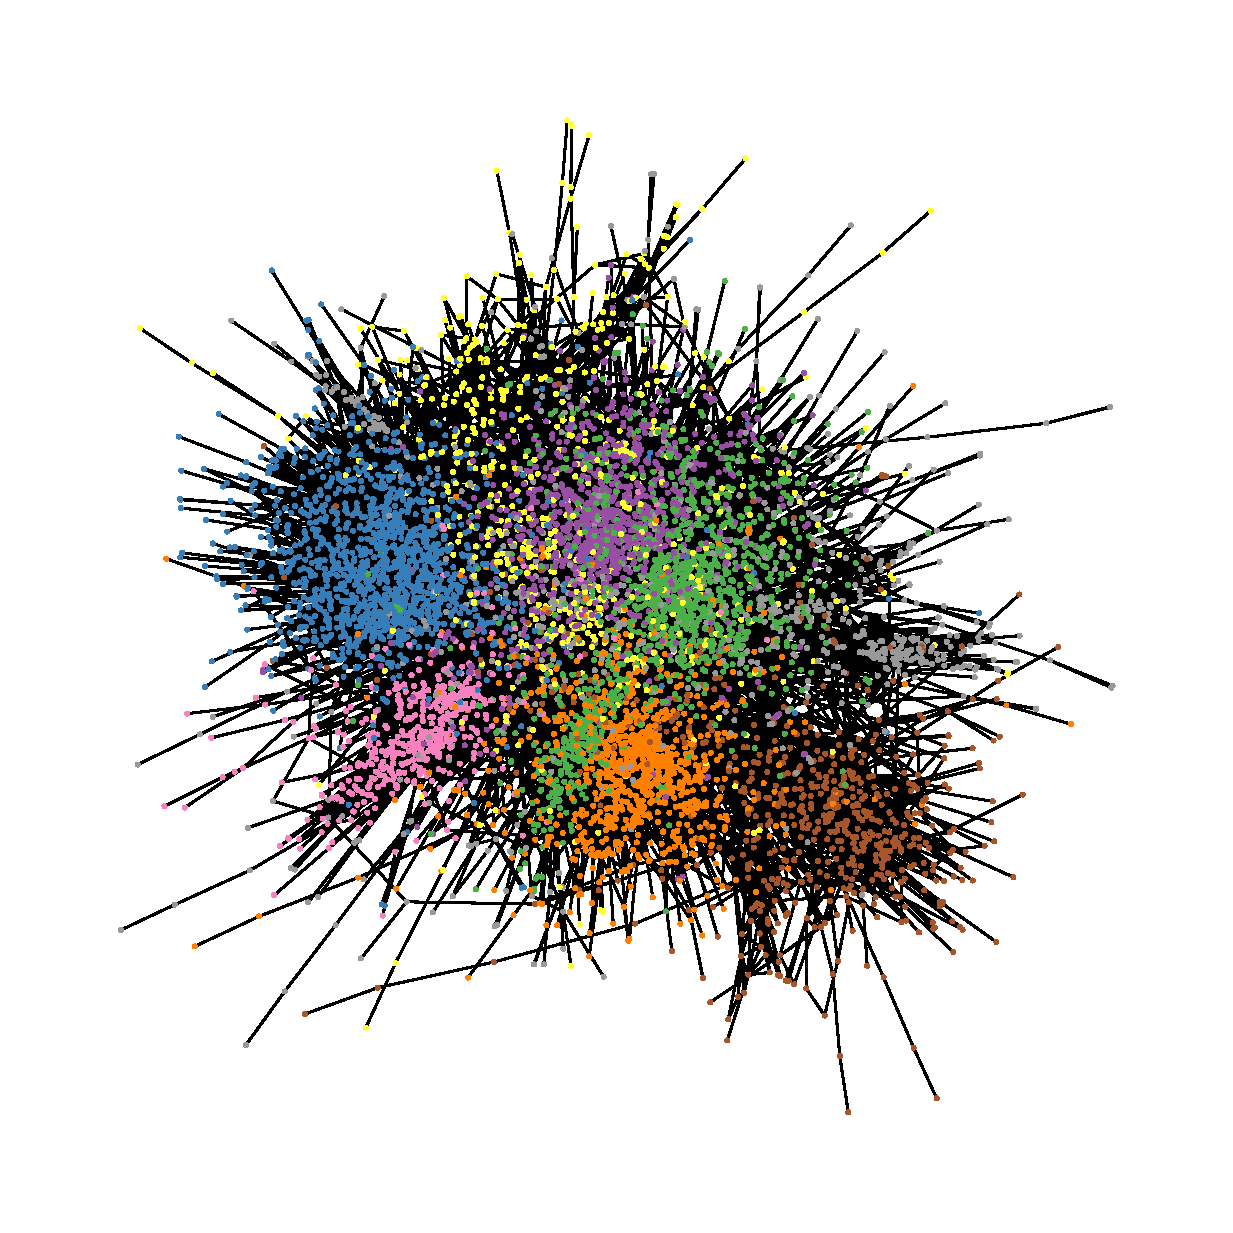
\includegraphics[width=0.5\linewidth]{figures/Qgreedy聚类结果}
	\caption{Qgreedy聚类结果}
	\label{fig:Qgreedy}
\end{figure}

\section{文本分析——J.R.R.Tolkien奇幻小说分析}
\subsection{J.R.R. Tolkien奇幻小说简介}

约翰·罗纳德·鲁埃尔·托尔金,CBE(英语:John Ronald Reuel Tolkien,常缩写为J.R.R.Tolkien,1892年1月3日-1973年9月2日),英国作家、诗人、语言学家及大学教授,以创作经典古典奇幻作品《霍比特人》、《魔戒》与《精灵宝钻》而闻名于世。\cite{Tolkien}

本章节选用经典的《精灵宝钻》《霍比特人》《魔戒》共三部主要作品进行分析。三部作品分别讲述了第一纪元众神创造世界、精灵族巧匠费艾诺打造精灵宝钻、诺多族为夺回精灵宝钻而开始征战米尔寇的悲情故事;第二纪元人类兴起、战胜米尔寇(魔苟斯)的奇幻史诗;以及第三纪元索隆意图统治世界以及相关的征战历史。

\subsection{数据处理以及词云绘制}

首先利用jieba对原文进行分词,去掉停用词表中的停用词以及所有标点符号、长度等于1的词,基于这些数据绘制词云图,如图\ref{fig:词云图}。图中弗罗多、山姆、甘道夫、阿拉贡等均为主要人物。
\begin{figure}[tbph!]
	\centering
	
\includegraphics[width=0.5\linewidth]{figures/词云}
	\caption{词云图}
	\label{fig:词云图}
\end{figure}

\subsection{词语相似性分析}

对原文用正则表达式进行拆分,分成若干个章节,之后分别构建词袋模型、2-gram共现矩阵以及Word2vec模型进行分析,最终结果如表格\ref{tab:最相近的词}。其中词袋模型和2-Gram模型结果更令人满意:如费艾诺被识别出了相近词“诺多族”,表明费艾诺是诺多族领袖、“菲纳芬”、“芬威”等都是费艾诺的亲属,“雅语”应为“昆雅语”,代表费艾诺使用这种语言、并且亲自改造了这种语言;“巫师”代表甘道夫在中土大陆的身份是巫师、“阿拉贡”、“弗罗多”是与甘道夫密切相关的人物;“至尊”来源于“魔戒至尊”这句邪恶的咒语以及“至尊魔戒”这个人们对他的称呼、“销毁魔戒”是《魔戒》的一个主线;“九戒”是屈从于至尊魔戒的九枚戒指。可见词袋模型、2-Gram模型效果比较理想。而Word2Vec模型效果不理想,这些“相近词”在原文中和这些人物没有明显关联。
% Please add the following required packages to your document preamble:
% \usepackage{multirow}
\begin{table}[!htbp]
	\centering
	\begin{tabular}{l|l|ll|l}
		\hline
		指标词                  & 词袋模型 & \multicolumn{2}{l|}{2-Gram} & Word2Vec \\ \hline
		\multirow{5}{*}{费艾诺} & 诺多族  & 雅语             & 母名         & 唱到       \\
		& 艾诺   & 芬威             & 雅语         & 山毛榉      \\
		& 但费   & 那座             & 岛屿         & 武装       \\
		& 菲纳芬  & 海岸             & 他们         & 欧西       \\
		& 愚行   & 家园             & 海湾         & 不想       \\ \hline
		\multirow{5}{*}{甘道夫} & 巫师   & 成为             & 市长         & 羽箭       \\
		& 需要   & 阿拉贡            & 抵达         & 一间       \\
		& 现在   & 13             & 弗罗多        & 打碎       \\
		& 已经   & 远征队            & 抵达         & 沉默       \\
		& 知道   & 成为             & 河谷         & 呼姆       \\ \hline
		\multirow{5}{*}{魔戒}  & 至尊   & 页数             & 参考         & 这才       \\
		& 销毁   & 阿美             & 洛斯         & 抱        \\
		& 这枚   & 无声             & 辅音         & 格        \\
		& 九戒   & sirion         & 瑞安         & 地面       \\
		& 泅水   & 更为             & 美观         & 有过       \\ \hline
	\end{tabular}
	\caption{最相近的词}
	\label{tab:最相近的词}
\end{table}

\subsection{利用深度学习进行小说创作}

《胡林的儿女》是《精灵宝钻》故事背景下的一个小故事,因为此传奇较为出彩而被整理专门出版,本部分试图通过深度学习模型模仿作者的行文风格来续写《胡林的儿女》。

本节用到的深度学习模型为LSTM模型。在数据处理方面主要进行了如下操作:首先载入原始数据,之后利用jieba进行分词,获取词频最高的若干词汇,再将词频最高的若干词汇专门留下,剩下的词拆成单个字,从而构建一个词库数据集。将该数据集带入LSTM进行训练,并利用胡林的儿女原文的第一段作为意境生成器,对训练的模型进行意境提取,并以“刚多林的陷落”作为开头续写文章;首段数据集如下:

“图奥出身的那支民族在森林里、高地上游荡,他们不知道也不歌颂大海。不过,图奥不和他们一起生活,而是独自住在一座名叫米斯林的湖附近,有时在湖畔的林中打猎,有时在岸边用他以熊筋和木头做成的简陋竖琴弹奏乐曲。众人听说他那粗犷的歌声含有力量,纷纷从远近前来听他弹唱,但是图奥不再歌唱,动身去了偏僻荒凉的地方。他在那里见识了诸多新奇的事物,并且从流浪的诺多族那里学到了他们的语言与传承学识,但他命中注定不会永远留在那片森林中。”

训练30个epoch之后的模型生成结果如下:

刚多林的陷落,他们在那里,他们的力量都是在中洲的土地上,他们的力量都是在中洲的土地上,他们的力量都是在中洲的土地上,他们的力量都是在中洲的土地上,他们的力量都是在中洲的土地上,他们的力量都是在中洲的土地上,他们的力量都是在中洲的土地上,他们的力量都是在中洲的土地上,他们的力量都是在中洲的土地上,他们的力量都是在中洲的土地上,他们的力量都是在中洲的土地上,他们的力量都是在中洲的土地上,他们的力量都是在中洲的土地上,他们的力量都是在中洲的土地上,他们的力量都是在中洲的土地上,他们的力量都是在中洲的土地上,他们的力量都是在中洲的土地上,他们的力量都是

训练50个epoch之后:

刚多林的陷落,他们的子民都是在中洲的世界里,他们的力量也是,他们的力量都是在中洲的世界里,他们的力量也没有任何任何爪牙的人。他们的儿子们在那里,他们在那里,他们的子民都是在那里,他们的心生了。  “我的朋友们,”他说,“我想,我也不需要。”  “我的意思是:‘我的儿子们,我也不需要。”  “我的意思是:‘我的儿子们,我也不需要。”  “我的意思是:‘我的儿子们,我也不需要。”  “我的意思是:‘我的儿子们,我也不需要。”  “我的意思是:‘我的儿子们,我也不需要。”  “我的意思是:‘我

可以看到两次写作的结果都不理想,30个epoch之后只能重复说一些话;50个epoch之后写作内容似乎是胡林在发泄对儿子不争气的愤怒心情,在写作能力上比30个epoch之后好很多。


%Complete the assignment now
% *** REFERENCES ***
\newpage
\bibliography{bibliography}
\bibliographystyle{naturemag}
\end{document}
%%%%%%%%%%%%%%%%%%%%%%%%%%%%%%%%%%%%%%%%%%%%%%%%%%%%%%%%%%%%%%%%%%
%%%%%%%%%%%%%%%%%%%%%%%%%%%%%%%%%%%%%%%%%%%%%%%%%%%%%%%%%%%%%%%%%%